\documentclass[12pt,a4]{article}\usepackage[]{graphicx}\usepackage[]{xcolor}
% maxwidth is the original width if it is less than linewidth
% otherwise use linewidth (to make sure the graphics do not exceed the margin)
\makeatletter
\def\maxwidth{ %
  \ifdim\Gin@nat@width>\linewidth
    \linewidth
  \else
    \Gin@nat@width
  \fi
}
\makeatother

\definecolor{fgcolor}{rgb}{0.345, 0.345, 0.345}
\newcommand{\hlnum}[1]{\textcolor[rgb]{0.686,0.059,0.569}{#1}}%
\newcommand{\hlstr}[1]{\textcolor[rgb]{0.192,0.494,0.8}{#1}}%
\newcommand{\hlcom}[1]{\textcolor[rgb]{0.678,0.584,0.686}{\textit{#1}}}%
\newcommand{\hlopt}[1]{\textcolor[rgb]{0,0,0}{#1}}%
\newcommand{\hlstd}[1]{\textcolor[rgb]{0.345,0.345,0.345}{#1}}%
\newcommand{\hlkwa}[1]{\textcolor[rgb]{0.161,0.373,0.58}{\textbf{#1}}}%
\newcommand{\hlkwb}[1]{\textcolor[rgb]{0.69,0.353,0.396}{#1}}%
\newcommand{\hlkwc}[1]{\textcolor[rgb]{0.333,0.667,0.333}{#1}}%
\newcommand{\hlkwd}[1]{\textcolor[rgb]{0.737,0.353,0.396}{\textbf{#1}}}%
\let\hlipl\hlkwb

\usepackage{framed}
\makeatletter
\newenvironment{kframe}{%
 \def\at@end@of@kframe{}%
 \ifinner\ifhmode%
  \def\at@end@of@kframe{\end{minipage}}%
  \begin{minipage}{\columnwidth}%
 \fi\fi%
 \def\FrameCommand##1{\hskip\@totalleftmargin \hskip-\fboxsep
 \colorbox{shadecolor}{##1}\hskip-\fboxsep
     % There is no \\@totalrightmargin, so:
     \hskip-\linewidth \hskip-\@totalleftmargin \hskip\columnwidth}%
 \MakeFramed {\advance\hsize-\width
   \@totalleftmargin\z@ \linewidth\hsize
   \@setminipage}}%
 {\par\unskip\endMakeFramed%
 \at@end@of@kframe}
\makeatother

\definecolor{shadecolor}{rgb}{.97, .97, .97}
\definecolor{messagecolor}{rgb}{0, 0, 0}
\definecolor{warningcolor}{rgb}{1, 0, 1}
\definecolor{errorcolor}{rgb}{1, 0, 0}
\newenvironment{knitrout}{}{} % an empty environment to be redefined in TeX

\usepackage{alltt}

% ---- Metadata ---- %

\title{Honesty by Convenience: Corruption Tolerance in Ecuador}
\author{Daniel Sánchez}
\date{June 2022}

% ---- Load Packages ---- %

% Math

\usepackage{savesym} % Need to "save" the command that is already defined \varTheta

\usepackage{amsmath}
  \savesymbol{varTheta} 

% Fonts

% To set the TNR font for both text and equations:

\usepackage{mathspec}
  \setallmainfonts(Digits,Greek,Latin){Times New Roman}
\restoresymbol{MTP}{varTheta}

% Formatting

\usepackage{setspace} % Double spacing
  \doublespacing

\usepackage[margin = 1in]{geometry} % 1 inch margin

\usepackage{lscape}

\setlength{\parindent}{0pt} % No indent

% Setting the size of the section titles

\usepackage{titlesec}

\titleformat*{\section}{\normalsize\bfseries}

% Citation & Bibliographies

\usepackage[backend = biber, style = apa, citestyle = apa]{biblatex}
  \addbibresource{references.bib}
  
% For tables:

 % For the modelsummary tables:
\usepackage{siunitx}
\usepackage{booktabs} 
  \newcolumntype{d}{S[input-symbols = ()]}
\usepackage{multirow}
\usepackage[flushleft]{threeparttable}

% For figure and table captions

\usepackage{caption}
  \captionsetup{labelfont = bf} % All in bold  
  
% Other packages

\usepackage{csquotes} % For quotation marks

\usepackage{epigraph} % For epigraph
  \setlength\epigraphwidth{9cm}
  \setlength\epigraphrule{1pt}

\usepackage{float} % For the H float option- only used in emergencies (lol)

\usepackage{textcomp} % For the registered trademark symbol.

% Always load these packages at the end of the preamble:

\usepackage{hyperref}

% ---- R Stuff to be used in the whole document ----

% Here I will execute or source R code through chunks that I need to use throughout the whole document.

% General settings



% Load the data by sourcing the data manipulation script. Note that survey design objects are indeed created in this script.
% We use the time argument in the chunks to reread or rerun the chunk in case external files are updated and chunks need to be rerun and re-cached.


% Perform all survey-robust tabulations by sourcing the R Script. 
% These are used on the text later.


% Run the first models


\IfFileExists{upquote.sty}{\usepackage{upquote}}{}
\begin{document}

% ---- Sections ---- %

% Abstract Child Document


% Abstract .Rnw File


\begin{center}
\textbf{
Honesty by Convenience: Corruption Tolerance in Ecuador\\
Daniel Sánchez}
\end{center}

\textit{
Attitudes towards corruption may be a strong determinant of its incidence. Using survey
data from the AmericasBarometer, binary-outcome empirical models are estimated to discover
the key determinants of an increase in corruption tolerance in Ecuador between 2014 and
2016. It is found that two key variables may have influenced this increase. People who approved
of the President’s job performance were initially less likely to justify bribes yet by 2016 they started justifying corruption more. Those who identified closer to the political right justified it more in 2016 as well. The increase is explained through these variables as the percentage of people who approved the President's performance decreased and the percentage of people identified with the political right increased. It is also found that the people who were either employed or outside the labor force justified corruption more in 2016 when compared to those who were unemployed.}

% Introduction Child Document


% Introduction .Rnw File

\section{Introduction}

% Corruption Tolerance Choropleth Map based on 2019 values

% Sorry, this map was done with the paid AmericasBarometer databases, so I cannot actually put my source code and have it executed by KNITR. USFQ students are free to access another version of the document, they must only email me. Third parties must wait until I do it with the free databases. Check out hbc-v2 for some more info.

\begin{figure}[htbp!]
    \begin{center}
    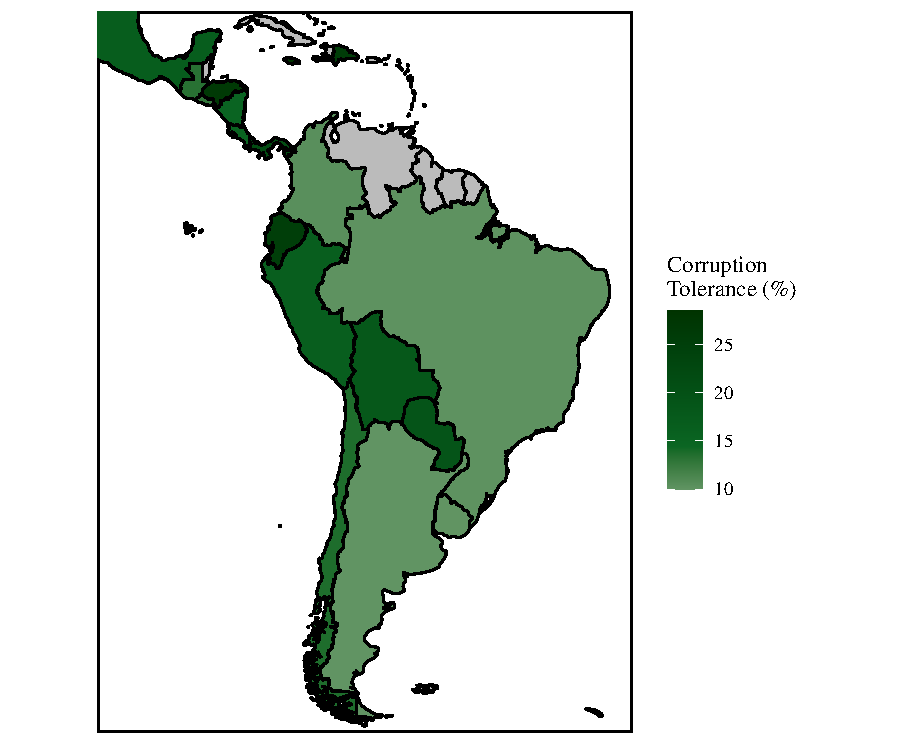
\includegraphics[scale = 0.6]{images/ctol_map.pdf}
    \end{center}
    \caption{Corruption Tolerance (\%) Choropleth Map in 2019}
    \label{fig:ctolmap}
A choropleth map showing corruption tolerance percentages across Latin America in 2019, where Ecuador places third in the most corruption tolerant countries. Data from the \textregistered AmericasBarometer 2018/19. 
\end{figure}

\enquote{Even if you are from [my political party], I will fulfill my duties. If you steal, steal well!  Justify well! But do not let your affairs be seen, comrades} \footnote{Translated from Cerda, 2021 in \cite[para. 2]{PlanV.2021}}. Uttered publicly by Rosa Cerda, Ecuadorian congresswoman for the Napo province \parencite{Castro.2021}, these comments met widespread criticism around the country, although the remarks were initially met by cheers from the audience she addressed. However, Cerda's declarations did not transcend an eight day suspension \parencite{Ordonez.2021} and the whole event was soon forgotten by most citizens. 

This episode is only one of many corruption-related scandals that have happened in Ecuador, a middle-income country in South America. The country has seen increased COVID-19 vaccine inequality \parencite{Taj.2021}, weakened public health services \parencite{Celi.2020}, policymakers charging fees for political positions \parencite{Espinosa.2021}, lost Social Security funds \parencite{Pesantes.9152020}, a former president convicted \parencite{Valencia.2020} as well as two vice-presidents impeached and removed on charges of corruption \parencite{Cabrera.2020}, among others. However, it is almost as if these no longer cause outrage: at most, they cause a sigh of disappointment or social media outrage which dwindles shortly after.

This apparent ambivalence has seen Ecuador place well above the corruption median in the world according to both Transparency International's and the World Bank's corruption indexes. About 90\% of voting-age Ecuadorians believe that at least half of politicians are corrupt and more than a quarter of them admit having been involved with bribes in 2019, according to the AmericasBarometer (AB) survey by the Latin American Public Opinion Project (LAPOP). However, a mere 8.08\% consider that corruption is the most serious problem faced by the country and in fact 25.38\% of Ecuadorians believe that paying a bribe is justified. Tolerance to corruption has risen 11.79 percentage points from 2014 to 2019. Furthermore, Figure \ref{fig:ctolmap} shows that Ecuador is also one of the countries with the highest corruption tolerance in the region.

This paper aims to investigate the determinants of the largest corruption tolerance increase in Ecuador from 2014 to 2016, as shown by Figure \ref{fig:ctoly}. This period coincided with two key events. First, the popularity of the governing regime sharply dropped for the first time in a decade \parencite{Quillupangui.2016}. Second, the country faced an economic recession \parencite{Weisbrot.2017}. The present paper will seek to investigate the increase's determinants by estimating binary-outcome models through logistic regression, which relates the probability of tolerating corruption to several individual-level public opinion and economic indicators. Survey-data from the AmericasBarometer is used for the empirical modelling. It is determined that changes in presidential job approval as well as in political wing preferences during 2014 and 2016 could have influenced the increase. It is also found that those not unemployed (employed or outside the labor force) justified corruption more in 2016 relative to those who were unemployed.

% Corruption Tolerance Time Series Graph

\begin{figure}[htbp!]
\begin{knitrout}
\definecolor{shadecolor}{rgb}{0.969, 0.969, 0.969}\color{fgcolor}

{\centering 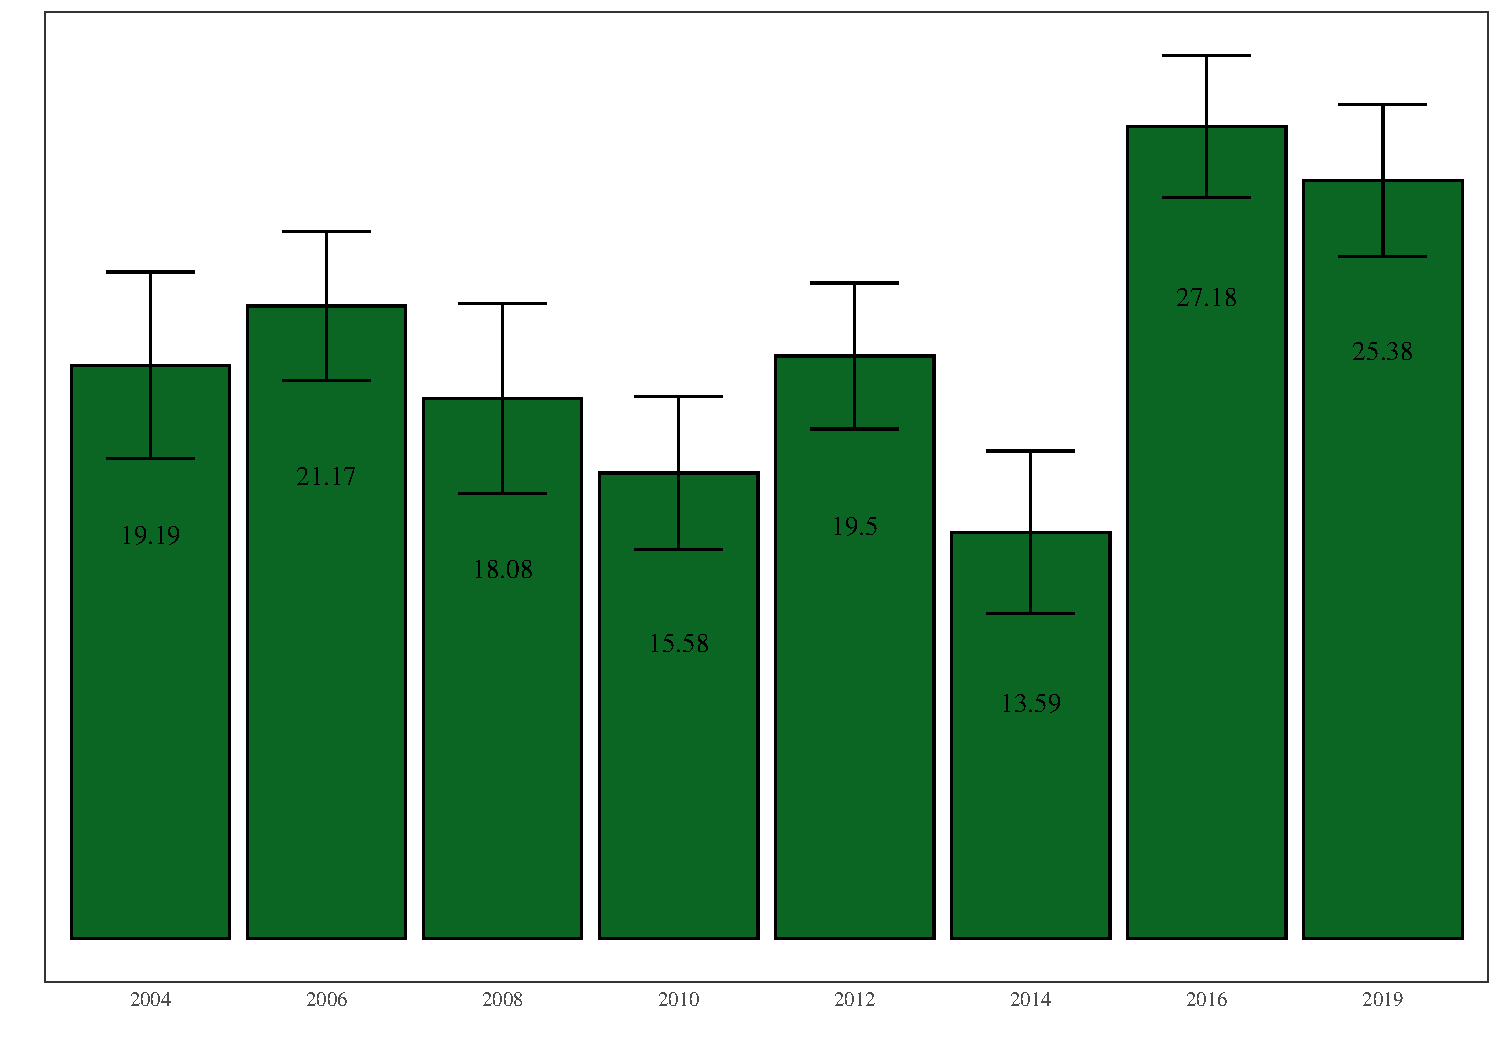
\includegraphics[width=\maxwidth]{figure/ctol_graph-1} 

}


\end{knitrout}
\caption{Percent of Ecuadorians who justify corruption, by year}
\label{fig:ctoly}
The evolution of corruption tolerance in Ecuador. Error bars show design-adjusted 95\% confidence intervals.
\end{figure}

Changes in attitudes toward corruption can be important for studying corruption incidence as a higher degree of corruption tolerance will eventually lead to more corruption \parencite{Campbell.2014, Ariely.2019}. Learning what drives corruption tolerance can then foster better policymaking and citizen attitudes which steers individuals away from dishonest acts. The rest of the paper proceeds as follows. The following section gives an economic and political background of the paper's setting, Ecuador. Section \ref{sec:background} reviews the relevant literature. Section \ref{sec:methodology} explains the empirical methodology. Section \ref{sec:results} presents and discusses the results from the estimation of empirical models. Section 7 concludes. 

% Institutional Background Child Document


% Context .Rnw File

\section{Economic and Political Background}
\label{sec:background}

Ecuador is a middle income country located in upper South America next to Colombia and Peru. Its GDP for 2022 is projected to be 115.47 billion US dollars, with an expected growth rate of 2.68\% \footnote{Data is from the IMF's World Economic Outlook dataset for October 2022.} Its population size notwithstanding, Ecuador is a naturally and ethnically diverse country, yet seems to be anchored to issues that have tormented it since its beginnings as a nation. \textcite{FederalResearchDivision.1991} identified four key issues have determined the social and economic trajectories of the country: (i) a skewed social structure, (ii) persistent regional rivalries, (iii) a considerable dependence on oil (iv) a lack of strong political institutions (p. xxi). In late 2022, these issues still dominate much of Ecuador's political and social environment. Since the corruption tolerance increase took place during a key period where two of these issues were most apparent, it is important to briefly review these mechanisms.

Ecuador's modern economic history can be traced back to the late 1960's: the finding of petroleum fields in the Ecuadorian Amazon in 1967, as well as its nationalization in the following years \parencite{EmpresaPublicaPetroEcuador.2013}. The economy grew at rates never seen before, which led to important social and economic transformations in Ecuadorian society \parencite{Hurtado.2007, FederalResearchDivision.1991}. The nationalization of oil greatly increased public revenues, which allowed for expansionary fiscal policy and overall growth. Unfortunately, this became a double-edged sword as it increased Ecuador’s dependency in global market price fluctuations since fiscal policy became tied to the ability to sell oil at a high price. Regardless of the public investment, the country has been an underdog in economic terms as its GDP per capita has stagnated whereas comparable South American nations have seen considerable growth, especially after 1990. An economic crisis in the late 90's led the country to its official dollarization, which reduced further the government's role in managing the economy as monetary policy was no longer a possibility. 

Political instability interacted with the dependence on commodity prices to hinder growth. The modern political history of the country starts in 1979, when the population was able to break a decade-long series of dictatorial regimes by electing a new president and a new constitution. However, the return to democracy did not stability: between 1979 and 2006, the country had 12 presidents and on average, Ecuador sees major protests against the government every 6 years \parencite{Loaiza.2022}. This constant political instability disallows for the establishment of long-term economic policies that can address the unhealthy dependence on commodities.

In 2006, a left-leaning government was elected, which concentrated power in the executive branch and engaged in significant reform through public spending. This government enjoyed high approval ratings for most of its tenure until 2016, as seen in Figure \ref{fig:ecua_pol}. The key was the leader, rather than the party or its ideals:  branding himself as \enquote{the biblical underdog} \parencite[para. 4]{Hedgecoe.2009}, charismatic academic Rafael Correa distanced himself from the country's political elite and constantly denounced corruption and injustice in the system. The new government promised a radical change in 2007 and did deliver in a way as it gave Ecuador a politically stable though totalitarian environment, as well as other changes in political and economic mechanisms \parencite{Weisbrot.2017}. 

% Create the data to be used for the political opinion variables:

% Now do the graph
\begin{figure}[htbp!]
\begin{knitrout}
\definecolor{shadecolor}{rgb}{0.969, 0.969, 0.969}\color{fgcolor}

{\centering 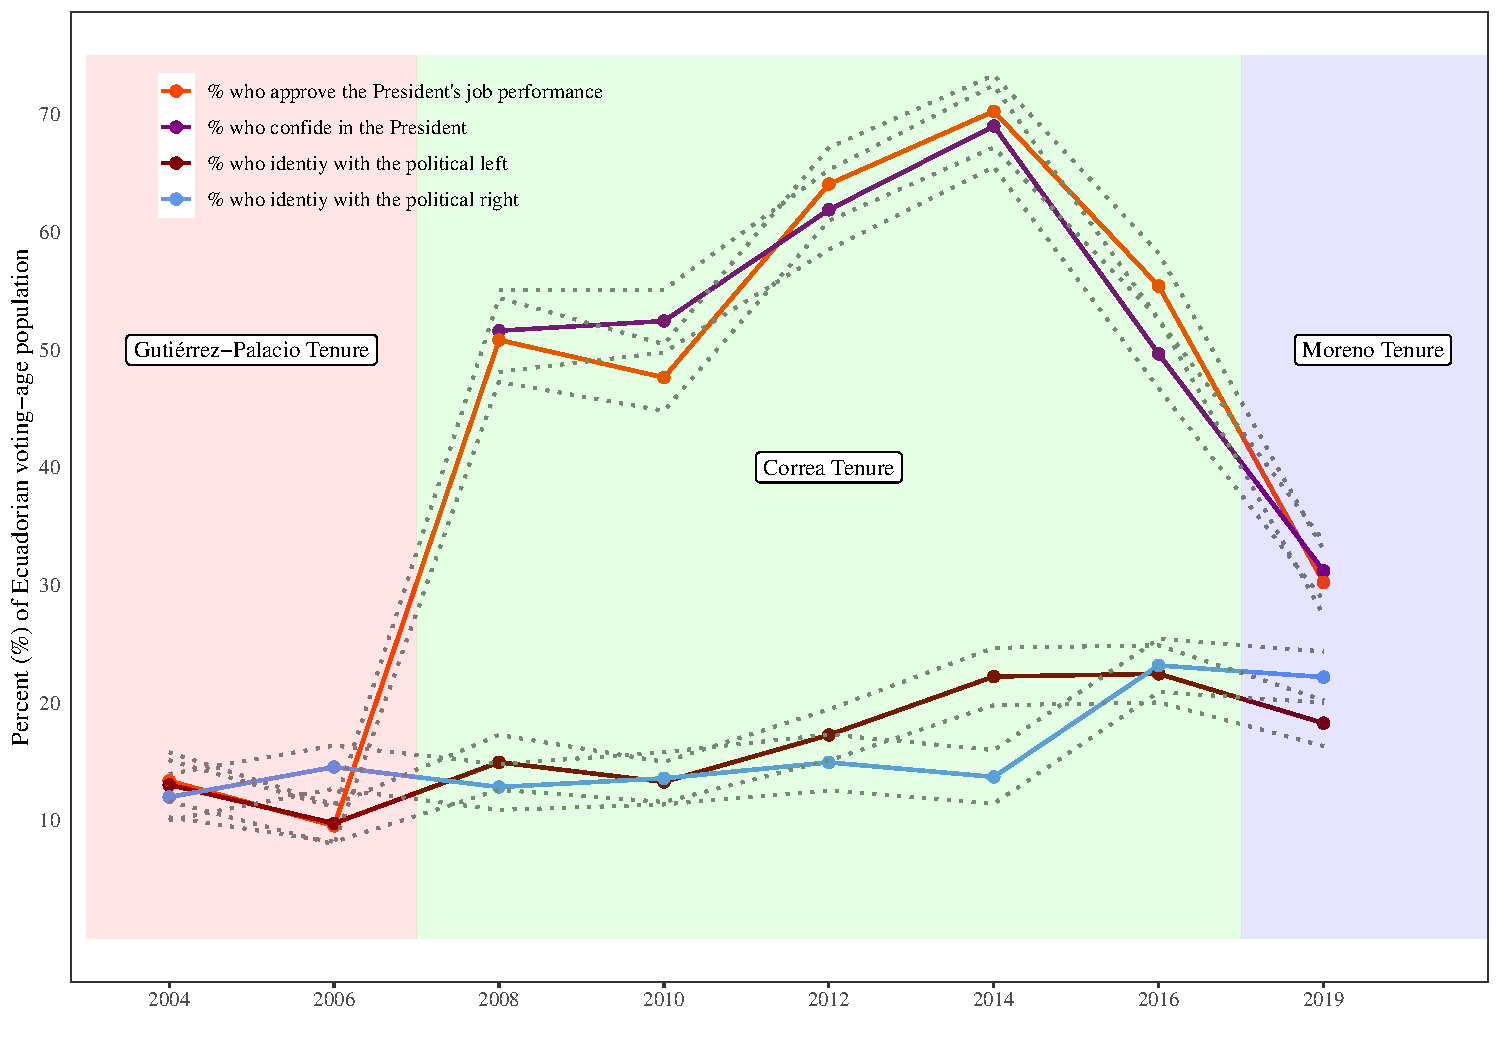
\includegraphics[width=\maxwidth]{figure/political_graph-1} 

}


\end{knitrout}
\caption{Ecuadorian public opinion indicators, 2004-2019}
\label{fig:ecua_pol}
Time series for political public opinion questions asked in the AB. Error bars show 95\% design-adjusted confidence intervals.
\end{figure}

Figure \ref{fig:ecua_pol} shows that the President reached an all-time high popularity in 2014 and then a severe drop in 2016. This is seen through the percent of people who approve the President's job performance and the percent who report confidence in him. Another notable change in the political landscape of this period is the way that voting-age population identified politically. There was a notable increase of the people who identified as the \enquote{right} of the political wings, while those who identified with the \enquote{left} did not see significant changes. 

The administration's high popularity allowed Correa to vanquish every political opponent: during most of his tenure there was no need of any kind of legislative pact to pass policy, as he enjoyed well over two-thirds majority in all political apparatuses. This government was often criticized due to its totalitarian practices yet the average Ecuadorian voter appeared deaf to this. Institutionality, democratic values, the separation of powers, etc. seemed awfully abstract and far from appealing to a traumatized nation. The new government was able to convince the people that it had been the political right who had destroyed the country, an idea that has haunted the current presidency of conservative businessman Guillermo Lasso, elected in April 2021.

As Ecuador entered a severe recession due to plunges in commodities’ prices and a fatal earthquake in 2016, the Correa administration was forced to take austerity measures, which were widely unpopular. Further, a significant amount of corruption accusations appeared against top government officials, which planted the seed of a deep investigation about a complex corruption scheme involving top government officials and large corporations \parencite{Villavicencio.2019}, which ended in a capture order for Correa in 2020. Several narratives started to be constructed by government officials to explain the flaws and accusations denounced at that point. These included reducing corruption accusations to \enquote{political persecution} or unfounded claims done because of upcoming elections \parencite{Melendez.2017}. 

Regarding the economic recession, \textcite{Orozco.2015} holds that although the commodity price collapse in 2008 was greater, there was little reduction in economic activity in 2008 as the country had greater possibilities of international financing and savings left over from past oil funds, which were used to keep government expenditure high. In 2016, savings had eroded and government debt had grown bigger, which saw the economy stagnate significantly. A politically weakened Correa left Ecuador for Belgium in 2017, after giving up power to his political successor, Lenín Moreno, who later turned his back on Correa.

Having understood these mechanisms, it is clear that Ecuador proves to be an excellent setting for studying the determinants of corruption tolerance. The economic and historical background have created a laboratory to study how people react to highly corrupted environments in the presence of exogenous shocks. Any kind of analysis about that the corruption tolerance increase during the 2014-2016 period must necessarily account for the events that happened at the time. In the next section, I analyze the related literature to construct a framework that will allow me to use these events as potential determinants for corruption tolerance at the individual level. 


% Literature Review Child Document


% Literature Review Rnw File


\section{Literature Review}

The literature on corruption mostly focuses on corruption incidence and how it may determine other economic and social outcomes. Lesser attention has been given to the corruption tolerance phenomenon, yet a key finding of this subset of the literature is that the more tolerance and exposure to corrupt acts, the more likely it is that these will spread across individuals. \textcite{Ariely.2019} discuss experimental findings which show that individuals that pay a bribe or are requested to pay one are more likely to behave dishonestly in subsequent ethical dilemmas. \textcite{Gino.2009} show that subjects more exposed to dishonest behaviors are more likely to engage in them. 

An empirical study of corrupt organizations by \textcite{Campbell.2014} shows that initial exposure to dishonest acts can reate an organizational culture which fosters the incidence of corruption among its members. The corrupt culture may change the behavior of otherwise honest individuals through social pressure, notably when philosophies which hold that \enquote{the ends justify the means} are viewed as the organization's core values. Specifically for the variable at hand, \textcite{Carlin.2013} proposes that \enquote{bribery has a self-perpetuating mechanism: if the rule of law is so weak that state actors are brazen enough to solicit bribes and self-interested citizens feel justified in paying them, the supply and demand of bribery will converge to form strong social behavioral norms.} (p.6). 

It is adequate to place corruption in a basic framework which will inform the empirical modelling, keeping two key channels in mind: the social and economic payoffs that corrupt acts imply. I build this framework based on the implications of a microeconomic model of corruption \parencite{Shleifer.1993}, the effect of social payoffs on economic outcomes \parencite{Akerlof.1980} and a behavioral theory of corruption normalization \parencite{Ashforth.2003}.

\textcite{Shleifer.1993} model bribes in a way where a public official trades public goods in exchange for bribes. Private agents then pay them to receive the good and the consumer surplus that any transaction brings. This might be understood as an individual economic incentive to engage in corrupt acts: paying the bribe allows the use of a desirable public good, or allows for quicker access to it. Thus, economic convenience could be an important determinant of how people behave around corruption: people may tolerate dishonesty if it means a positive economic payoff. 

On the other hand, there might be also moral considerations to the decision of tolerating or engaging in corruption. While the economic payoff of paying or receiving a bribe may be positive, the moral connotation of the act may bring shame or rejection from society. Avoiding a bad image can very well become an important determinant of the decision of engaging in corruption. Nevertheless, in environments where this is tolerated the negative social payoff of bribing might be smaller, which decreases the social payoff for being honest. \textcite{Akerlof.1980} holds that that social payoffs might change economic outcomes in a significant way, deviating from the neoclassical equilibria. How the social payoffs of corrupt acts are determined is key, as it could be assumed that most of the time the economic payoff of bribes is positive for the corrupt individual. 

\textcite{Ashforth.2003} develop a model to explain how corruption is normalized or tolerated in an organization, which helps to understand how these social payoffs are determined. The implications of this model imply that social payoffs of being corrupt should be decomposed in effects related to the institutionalization, rationalization and socialization of corruption.

Leadership in the organization is very relevant for institutionalization behaviors in Ecuador, considering its recent historical background. \textcite{Ashforth.2003} propose that leaders need not engage in corrupt acts to foster their normalization, they can simply facilitate or ignore the initial corrupt acts to have subordinates start normalizing corruption. Subordinates do not second-guess their superiors' decisions due to the habit of obedience, which is more prevalent in highly hierarchical organizations.

Two other mechanisms are involved in the normalization of corruption. The \textit{rationalization} mechanism of corruption is especially important, as it can be easily modelled at the individual level. This mechanism involves corrupt individuals rationalizing corruption in a way that they \enquote{avoid the adverse effects of an undesirable social identity} \parencite[p.13]{Ashforth.2003}. Relevant to the present context is the \textit{denial of responsibility} rationalization, in which corrupt individuals become convinced that they have no choice but to engage in corrupt acts due to external circumstances.  Denial of responsibility also involves individuals seeing their own corruption as a form of retribution against unfair previously exerted on them. Another denial of responsibility is when corrupt acts are justified because actors perceive those that denounce corruption as illegitimate authorities, charged with motives other than the well-being of the organization.

The socialization mechanism is concerned with the peer effects of corruption, where dishonest practices are \enquote{taught} to organization newcomers. Newcomers will be initially induced to change their attitudes towards corrupt beliefs, then being peer-pressured to escalate these practices. Since newcomers strive to be accepted, they end up adopting these dishonest behaviors as their own, while they also rationalize it to avoid the social costs of being dishonest. Later the newcomers become the ones that exert peer pressure on future members.

Having established a framework which will allow for better modelling of corruption tolerance, it is useful to look at what the literature has found with the variable at hand. \textcite{Singer.2016} find that for every country in Latin America in 2014, at least 60\% of the respondents perceive their governments to be corrupt but a much smaller proportion considers corruption to be the most important problem in their countries. It is found that those who justify corruption are those who have been exposed to some kind of bribe in the past\footnote{The original wording by the authors in the AB reports is \textit{corruption victimization}. Here, this variable is referred to as \textit{corruption exposure}, to account for the possibility that the respondent can be either a victim of corruption by being forced to pay a bribe or the initial corrupt agent who offers to pay one.}. Other significant determinants of corruption tolerance in 2014 were age and the urban-rural dichotomy. Younger participants tend to justify corruption to a higher degree, a finding robust through time and across countries of the region. Those living in rural settings also tend to justify corruption more.

\textcite{Lupu.2017} shows that corruption tolerance has been growing consistently in the region and that the average Latin American country has about a fifth of its population believing that corruption is justified. Between 2014 and 2016, corruption tolerance grew from 17.4\% to 20.5\% in the region. It is found that older citizens as well as those exposed to corruption before are more prone to justify it. The level of perceived corruption also appears as a significant determinant. \textcite{Lupu.2017} arrive to the conclusion that corruption may have become a \enquote{a self-fulfilling prophecy: as more and more citizens perceive that corruption is more widespread, they also become more likely to condone it}(p. 67). 

Regarding Ecuadorian corruption tolerance, \textcite{Moscoso.2018} find that corruption is also perceived to be widespread yet not regarded as an important problem. \textcite{Montalvo.2019} finds that the general trend for younger people to justify corruption more is also found in Ecuador. For the same round, \textcite{Moscoso.2020} find that besides age, interest in politics is a significant predictor as well as exposure to corruption, as found by \textcite{Lupu.2017} for the whole region. The empirical evidence can support corruption becoming a known inconvenience for daily life in the country rather than an unacceptable threat to the system, and that it is perceived as endemic to the political and social environments. 

% Methodology Child Document


% Methodology .Rnw File


\section{Methodology}
\label{sec:methodology} % Label the section to cross-reference later.

The AmericasBarometer (AB) survey from the Latin American Public Opinion project is used in this paper to investigate the corruption tolerance increase in Ecuador. This survey was administered in Ecuador and other Latin American countries from 2004 to 2019, at about two-year intervals. It asks about public opinion matters, including democracy, corruption, among others. The open-access AB databases available in the LAPOP \href{https://www.vanderbilt.edu/lapop/data-access.php}{website} are used for the empirical models. Table \ref{tab:descrip} presents descriptive statistics for all variables used.

% Here I will create a descriptive table including averages (and proportions) by year.
% This table is a bit difficult to construct because of its survey-weighted statistics and the rather complex structure, which is why I created it using Excel, exporting the results from calculations done in R.
\begin{table}[htbp!]
\onehalfspacing
\begin{center}
\caption{Descriptive statistics for all variables}
\label{tab:descrip}
\begin{tabular}{llcccc}
\toprule
\multicolumn{1}{c}{\multirow{2}{*}{Variable}} & \multirow{2}{*}{\begin{tabular}[c]{@{}l@{}} Question code \end{tabular}} & \multicolumn{2}{c}{2014}  & \multicolumn{2}{c}{2016}  \\ 
\cmidrule(l{3pt}r{3pt}){3-4} \cmidrule(l{3pt}r{3pt}){5-6}
\multicolumn{1}{c}{}                          &                                                                                         & Est. & SE & Est. & SE \\ \midrule
Corruption tolerance                          & EXC18                                                                                   & 13.59    & 1.39           & 27.18    & 1.21           \\
Unemployment                                  & OCUP4A                                                                                  & 10.06    & 1.04           & 22.89    & 1.2            \\
Confidence in the President                   & B21A                                                                                    & 69.01    & 1.77           & 49.64    & 1.49           \\
Approval of the President                     & M1                                                                                      & 70.26    & 1.57           & 55.41    & 1.43           \\
Economic situation (Worse)                            & IDIO2                                                                                   & 22.93    & 1.26           & 51.76    & 1.45           \\
No political wing                             & L1                                                                                      & 21.49    & 2.11           & 8.67     & 0.74           \\
Center                                        & L1                                                                                      & 42.58    & 1.92           & 45.7     & 1.49           \\
Left                                          & L1                                                                                      & 22.23    & 1.25           & 22.46    & 1.24           \\
Right                                         & L1                                                                                      & 13.7     & 1.16           & 23.17    & 1.15           \\
Women                                         & Q1                                                                                      & 50.37    & 0.34           & 50.29    & 0.3            \\
Age                                           & Q2                                                                                      & 39.41    & 0.17           & 38.64    & 0.22           \\
Years of education                            & ED                                                                                      & 10.67    & 0.15           & 11.43    & 0.14           \\
Urban                                         & UR                                                                                      & 65.21    & 4.11           & 66.41    & 4.07           \\
External political efficacy                   & EFF1                                                                                    & 35.31    & 1.69           & 41.93    & 1.33           \\
Internal political efficacy                   & EFF2                                                                                    & 38.55    & 1.58           & 41.49    & 1.34           \\
Participated in a protest                     & PROT3                                                                                   & 6.82     & 0.89           & 4.67     & 0.55           \\
Interest in politics & POL1 & 33.45 & 1.63 & 32.29 & 1.35 \\
Perceives corruption                          & EXC7, EXC7NEW                                                                           & 70.29    & 1.74           & 83.49    & 0.97           \\
Exposed to corruption                         & EXC 2,6,11,13,14,15,16                                                                  & 26.97    & 2.01           & 27.69    & 1.23           \\ 
\bottomrule
\end{tabular}
\end{center}
Descriptive statistics table with estimates (Est.) and robust standard errors (SE), where age, years of education and the external and internal political efficacies are arithmetic means. All other variables are percentages. Standard errors are adjusted for survey-design effects.
\end{table}

The empirical models estimated in this study will use the 2014 and 2016 rounds of the AB in Ecuador, with $n_{2014}=1489$ and $n_{2016}= 1545$. The survey is based on a multi-stage national probability design, with design-adjusted errors $\pm 2.5\%$ and $\pm 1.9\%$, respectively for each year (\cite{LAPOP.2014}; \cite{LAPOP.2017}). Both surveys are self-weighted, however, 95\% confidence intervals for the descriptive statistics which are adjusted for survey-design effects are presented when relevant. 

The empirical analysis is concerned with the \emph{EXC18} question: \enquote{Do you think given the way things are, sometimes paying a bribe is justified?} \parencite[p.96]{Moscoso.2018}, originally asked in Spanish. The question has been asked in all survey rounds in Ecuador and is the last one after a set of questions regarding corruption exposure and perception. This variable ($ctol$) is equal to 1 when the respondent answers \enquote{Yes}, 0 when the answer is \enquote{No} and dropped from the model otherwise. All models have $ctol$ as the explained variable and responses to other questions are used as regressors. 

In order to identify the changes in behavior which led to the increase, the survey rounds are pooled and the following general model is estimated: 

\begin{equation}
\label{eqn:genmod}
P(ctol = 1 | \textbf{\textit{X}} \hspace{0.04cm}) = G (\textbf{\textit{X}} \theta ) = G \left[ \beta_0 + \delta_0 y_{16} + \textbf{\textit{R}}'\beta + \delta_1 (y_{16} \cdot x^*) \right]
\end{equation}

where $\textbf{\textit{R}}$ is a vector of controls and $x^*$ is a key regressor whose change across time may have significantly influenced the rise of $ctol$ between 2014 and 2016. This key regressor is interacted with a year dummy, $y_{16}$, which equals unity for 2016 observations. The complete regressors' vector $\textbf{\textit{X}}$ includes all variables in $\textbf{\textit{R}}$, the key regressor $x^*$ and the interaction term. The parameters vector $\theta$ includes the vector $\beta$ as well as $\beta_0$, $\delta_0$ and $\delta_1$. $G$ is the link function; in this paper I follow the literature and use a logistic function as $G$. 

Consider the partial effect of the key regressor $x^*$ on $P(ctol =1| \textbf{\textit{X}})$:
\begin{equation}
\label{eqn:keype}
\dfrac{\partial P(ctol = 1 | \textbf{\textit{X}} \hspace{0.04cm})}{\partial x^*} = \dfrac{\partial G}{\partial \theta} \cdot 
\dfrac{\partial \theta}{\partial x^*} = \dfrac{\partial G}{\partial \theta} \cdot (\beta_{x^*}+ \delta_1 y_{16})
\end{equation}

The parameter $\delta_1$ would then measure the ceteris paribus effect of a change in the key regressor $x^*$ from 2014 to 2016 in $ctol$. Therefore, the coefficient of interest in this study is $\widehat{\delta}_1$. If there has been a change in 2016 in $x^*$ which significantly influences corruption tolerance, $\widehat{\delta_1}$ should be statistically significant. Further, a $\widehat{\delta}_1$ coefficient not statistically different from zero would mean that individuals with and without this key characteristic are equally likely to justify corruption across time. 

Average partial effects tables are shown for all models. I use survey-weighting to adjust for complex-survey design effects, as suggested by \textcite{Castorena.2021}. Since the sample is self-weighted, survey-weighting does not affect magnitudes, only standard errors.

% Results 1 Child Document


% Results I .Rnw File

\section{Results}
\label{sec:results}
As seen in Section \ref{sec:background}, two economic variables significantly changed during the corruption tolerance increase period: the percent of people who report a worse economic situation as well as unemployment. Variables which proxy attitudes in the political landscape also significantly changed: the percentage of people who confide in the President, the percentage who approve the President's performance and also the percentage of people who identified with the political right. These variables where used for simple empirical models, which follow the equation below.
\begin{equation}
\label{eqn:simplemod}
P(ctol = 1 | \textbf{\textit{X}} \hspace{0.04cm}) = G \left[ \beta_0 + \delta_0 y_{16} + \beta_1 x^* + \delta_1 (y_{16} \cdot x^*)\right]
\end{equation}
where the key regressor $x^*$ can be: a dummy variable set to unity for respondents who answered that their economic situation is worse (Model 1), a dummy variable set to unity for those who report being unemployed (Model 2), a discrete variable with numbers 1-7, where higher values imply a higher degree of confidence in the President (Model 3), a discrete variable with numbers 1-5, with higher numbers implying a higher rating of the President's job performance (Model 4) or a discrete variable with numbers from 1-10 where 1 is the extreme left and 10 is the extreme right (Model 5). 

Table \ref{tab:simplemodel} presents coefficients of the logistic model for Equation \ref{eqn:simplemod} and Table \ref{tab:apesimp} presents their associated average partial effects. It is shown that an unemployed person is 5.9\% more likely to justify corruption. Additionally, a respondent who answered one number higher for an increased degree of confidence in the President was 2.4\% less likely to justify it. Finally, a person who rated the President's job performance one unit higher was 4.4\% less likely to justify corruption. All other partial effects are not significant.

% Now, I'll make the table with modelsummary from the sourced stuff. 
\begin{table}[htbp!]
\caption{Logit coefficients for baseline models}
\label{tab:simplemodel}

\begin{tabular}[t]{lccccc}
\toprule
  & Model 1 & Model 2 & Model 3 & Model 4 & Model 5\\
\midrule
Constant & \num{-1.894}*** & \num{-1.989}*** & \num{-0.455}** & \num{0.553} & \num{-1.527}***\\
 & (\num{0.127}) & (\num{0.110}) & (\num{0.208}) & (\num{0.362}) & (\num{0.196})\\
2016 Dummy & \num{0.848}*** & \num{1.001}*** & \num{-0.188} & \num{-1.251}*** & \num{0.278}\\
 & (\num{0.158}) & (\num{0.132}) & (\num{0.238}) & (\num{0.415}) & (\num{0.234})\\
Worse Economic Situation & \num{0.131} &  &  &  & \\
 & (\num{0.169}) &  &  &  & \\
Unemployment &  & \num{1.015}*** &  &  & \\
 &  & (\num{0.205}) &  &  & \\
Confidence in President &  &  & \num{-0.288}*** &  & \\
 &  &  & (\num{0.037}) &  & \\
Approval of Pres. Performance &  &  &  & \num{-0.648}*** & \\
 &  &  &  & (\num{0.096}) & \\
Political Wing &  &  &  &  & \num{-0.047}\\
 &  &  &  &  & (\num{0.038})\\
Econ. Situation Interaction & \num{-0.025} &  &  &  & \\
 & (\num{0.197}) &  &  &  & \\
Unemployment Interaction &  & \num{-1.005}*** &  &  & \\
 &  & (\num{0.256}) &  &  & \\
Pres. Confidence Interaction &  &  & \num{0.206}*** &  & \\
 &  &  & (\num{0.044}) &  & \\
Pres. Approval Interaction &  &  &  & \num{0.568}*** & \\
 &  &  &  & (\num{0.111}) & \\
Pol. Wing Interaction &  &  &  &  & \num{0.095}**\\
 &  &  &  &  & (\num{0.043})\\
\midrule
$N$ & \num{2948} & \num{2950} & \num{2944} & \num{2941} & \num{2535}\\
AIC & \num{2893.64} & \num{2889.04} & \num{2848.57} & \num{2844.82} & \num{2574.81}\\
BIC & \num{2926.37} & \num{2920.98} & \num{2881.80} & \num{2876.65} & \num{2606.10}\\
\bottomrule
\end{tabular}


\vspace{0.15cm}
Logit coefficients of baseline models (Equation \ref{eqn:simplemod}) with design-adjusted std. errors. *$p$ < 0.1, **$p$< 0.05, ***$p$ < 0.01.
\end{table}

Consider the logit coefficients in Table \ref{tab:simplemodel}. The coefficient for the year dummy confirms the significance of the corruption tolerance increase in 2016, which is lost when considering interaction terms with confidence in the President, and actually has a negative sign with the other political variables. The inclusion of unemployment and economic situation do not eliminate the significance of the year dummy. Model 1 suggests that a person who reports having a worse economic situation does not tolerate corruption differently than those who report a same or equal economic situation. According to Model 2, respondents who were unemployed were more likely to justify corruption than those who were not \footnote{In this case, not being unemployed means either being employed, salary and hours worked notwithstanding, and also not being in the labor force (students, rentists, among others). Results are robust to including an employment variable.} The interaction term in this model has a negative sign, which shows that the effect of unemployment in 2016 was lower than in 2014, meaning unemployed people justified corruption less after political instability set in. 

% Do the APE table
\begin{table}[htbp!]
\caption{Average partial effects for logit models in Table \ref{tab:simplemodel}}
\label{tab:apesimp}

\begin{tabular}[t]{lccccc}
\toprule
  & Model 1 & Model 2 & Model 3 & Model 4 & Model 5\\
\midrule
2016 Dummy & \num{0.131}*** & \num{0.126}*** & \num{0.109}*** & \num{0.117}*** & \num{0.124}***\\
 & (\num{0.020}) & (\num{0.019}) & (\num{0.019}) & (\num{0.019}) & (\num{0.020})\\
Worse Economic Situation & \num{0.018} &  &  &  & \\
 & (\num{0.014}) &  &  &  & \\
Unemployment &  & \num{0.058}*** &  &  & \\
 &  & (\num{0.020}) &  &  & \\
Confidence in President &  &  & \num{-0.024}*** &  & \\
 &  &  & (\num{0.003}) &  & \\
Approval of Pres. Performance &  &  &  & \num{-0.044}*** & \\
 &  &  &  & (\num{0.008}) & \\
Political Wing &  &  &  &  & \num{0.003}\\
 &  &  &  &  & (\num{0.003})\\
\midrule
$N$ & \num{2948} & \num{2950} & \num{2944} & \num{2941} & \num{2535}\\
\bottomrule
\end{tabular}


\vspace{0.15cm}
Average partial effects for models in Table \ref{tab:simplemodel}, with design-adjusted std. errors. *$p$ < 0.1, **$p$< 0.05, ***$p$ < 0.01.
\end{table}

Models 3 and 4 display the same relationship: people who either trust or approve of the President in a higher degree also tolerate corruption less. A more zealous supporter of the regime believed bribes were not justified; however, this appears to change for 2016. The interaction terms for both variables are significant and positive: in 2016 supporters started to justify corruption more. This could explain the jump in corruption tolerance as regime support eroded in 2016, which meant that the number of non-supporters was higher and these respondents justified corruption more than supporters. Also, the supporters that remained started to justify bribes to a higher degree. In Model 3, the significance of the year dummy is lost, while in Model 4 the sign reversed.

The coefficients in Model 5 show that a person who identifies closer to the political right does not justify corruption more or less relative to those identifying closer to the political left. However, the interaction term shows that people answering higher values of this variable justified corruption more in 2016. Once again, the significance of the year dummy is lost when considering this variable. With a higher number of respondents identifying with the political right wing, who appear to justify corruption more, it would be understood how overall corruption tolerance increased.

% I need to draw the graph which shows the visual differences between groups and their corruption tolerance

% Now I do the data wrangling needed for this


% Now do the graph
\begin{figure}[htbp!]
\begin{knitrout}
\definecolor{shadecolor}{rgb}{0.969, 0.969, 0.969}\color{fgcolor}

{\centering 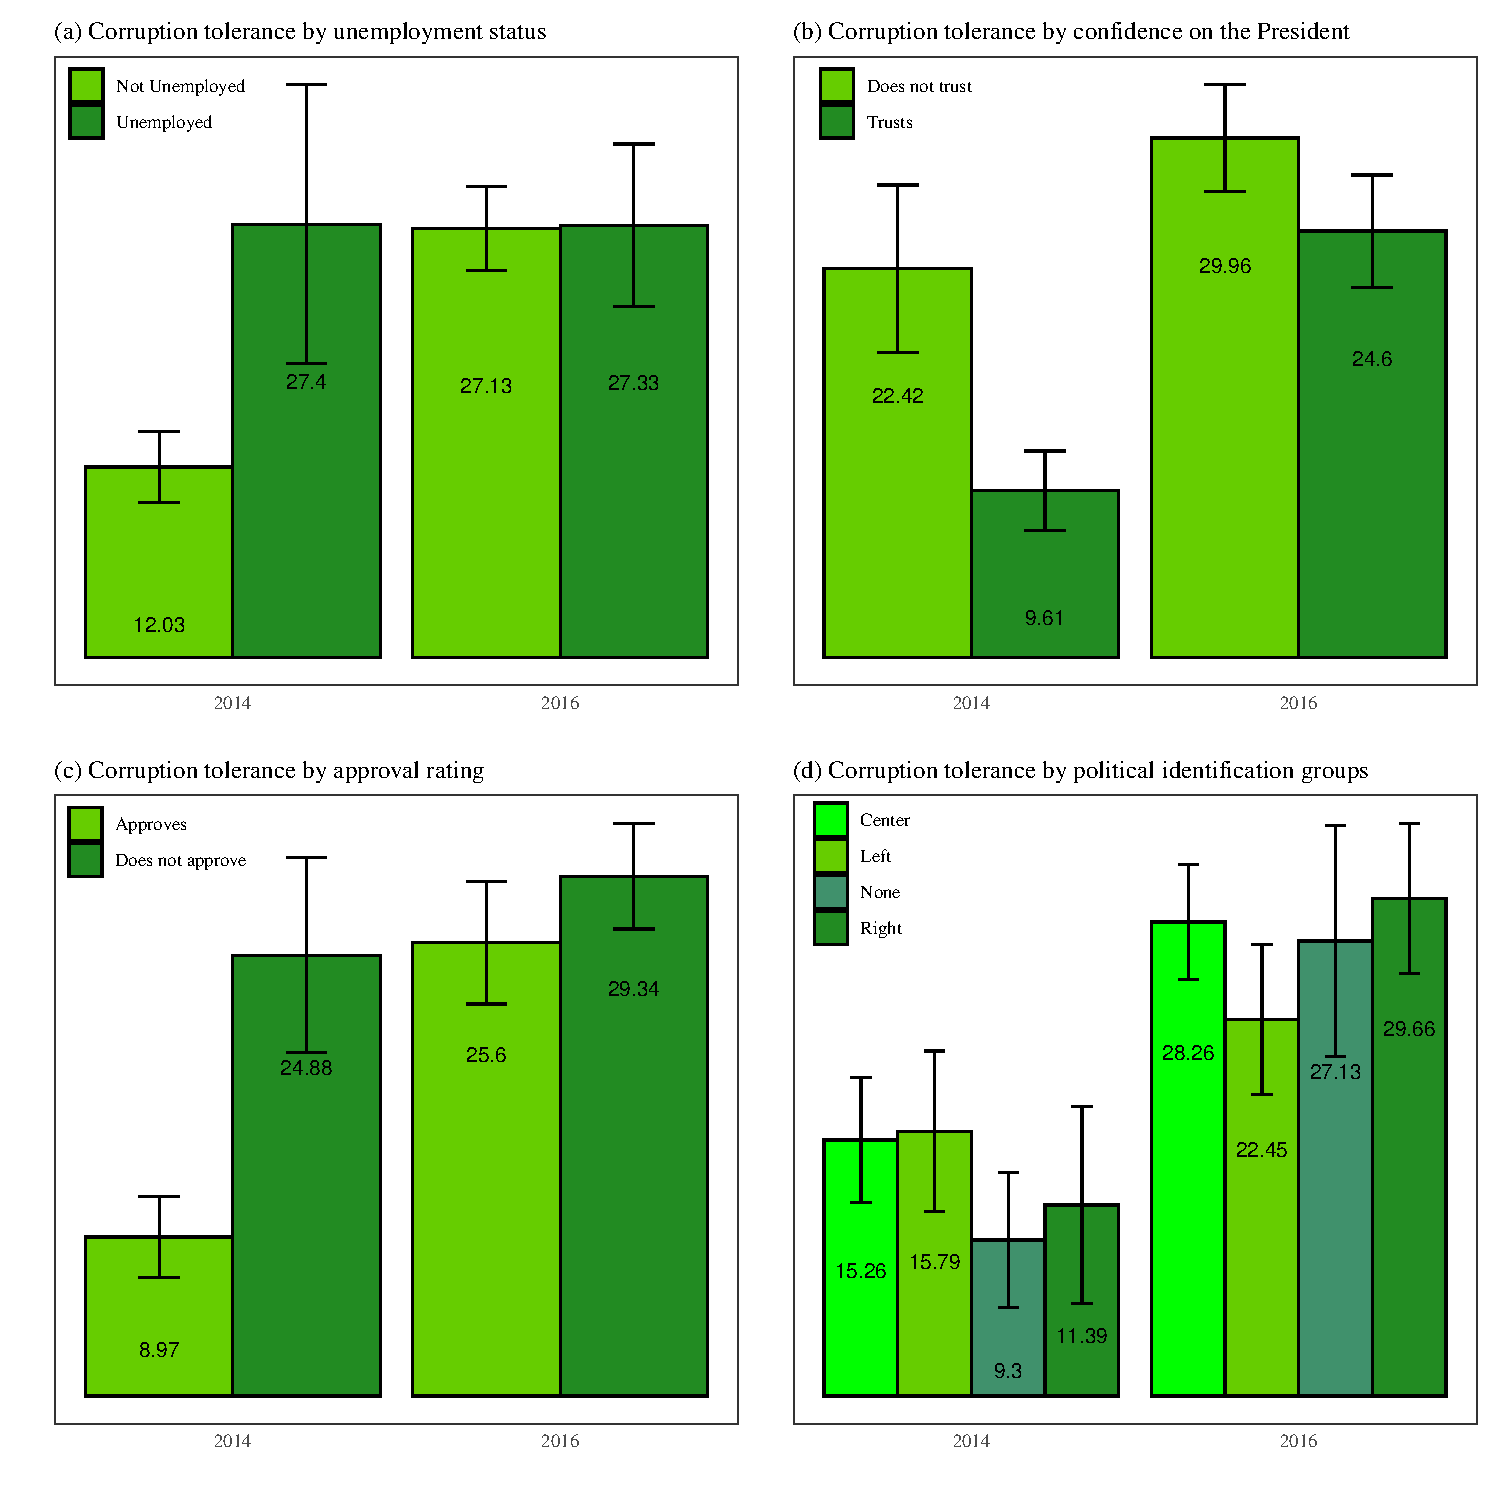
\includegraphics[width=\maxwidth]{figure/difgraph-1} 

}


\end{knitrout}
\caption{Graphical representations of corruption tolerance across key explanatory variables}
\label{fig:difgraph}
Figures show the percent that justify corruption across the groups used as explanatory models in Table \ref{tab:simplemodel}. Error bars represent the 95\% confidence intervals adjusted for design effects.
\end{figure}

These findings are supported by Figure \ref{fig:difgraph}. According to panel (a), in 2014, only 12.03\% of those not unemployed justified corruption, while in 2016 it increased to 27.03\%, very close to the percentage of unemployed people who justified it in 2016. The time difference between these point estimates is not statistically significant, which means that in 2016 the effect of unemployment in corruption tolerance approached zero. Thus, Figure \ref{fig:difgraph} along with Model 2 of Table \ref{tab:simplemodel} show that it was not the unemployed who started to justify corruption less, it was that the people who were not unemployed started to justify it more. Panels (b) and (c) of Figure \ref{fig:difgraph} show that the percentage of people who either confided in or approved the President and justified corruption increased significantly  between 2014 and 2016. This means that the negative effect of supporting the executive in 2016 was smaller than in 2014, as confirmed by the interaction term in Models 3 and 4 of Table \ref{tab:simplemodel}. In panel (d) of Figure \ref{fig:difgraph}, four different political groups are considered: the left, right, center and those who did not answer the question. All four groups saw increases in the percent of group members who justify corruption. All increases in corruption tolerance are significant, except for those who identify with the left wing. This is consistent with the coefficient sign seen in Model 5 for the political score variable. 


% Results 2 Child Document


% Results II .Rnw File


Now the general model as described by Equation \ref{eqn:genmod} is estimated with the key regressors as well as a set of controls at the individual level. I keep the variables which yielded statistically significant interaction tears with the year dummy in Table \ref{tab:simplemodeld} except for confidence in the president as job approval ratings contemplate the same effects. Coefficients are shown in Table \ref{tab:complexmod} and average partial effects are shown in Table \ref{tab:apescomp}. 

% Estimate the modified models, by sourcing that .R file


% Now create the table
\begin{table}[htbp]
\begin{center}
\caption{Logit coefficients for modified models}
\label{tab:complexmod}

\begin{tabular}[t]{lccc}
\toprule
  & Model 1 & Model 2 & Model 3\\
\midrule
Constant & \num{-0.674}* & \num{0.707} & \num{-0.351}\\
 & (\num{0.401}) & (\num{0.468}) & (\num{0.405})\\
2016 Dummy & \num{0.887}*** & \num{-1.217}** & \num{0.333}\\
 & (\num{0.145}) & (\num{0.477}) & (\num{0.252})\\
Woman & \num{0.124} & \num{0.136} & \num{0.127}\\
 & (\num{0.109}) & (\num{0.111}) & (\num{0.109})\\
Age & \num{-0.026}*** & \num{-0.026}*** & \num{-0.026}***\\
 & (\num{0.004}) & (\num{0.004}) & (\num{0.004})\\
Years of education & \num{-0.041}*** & \num{-0.038}** & \num{-0.039}**\\
 & (\num{0.015}) & (\num{0.015}) & (\num{0.015})\\
Lives in urban setting & \num{-0.020} & \num{0.013} & \num{0.009}\\
 & (\num{0.132}) & (\num{0.131}) & (\num{0.132})\\
External political efficacy & \num{-0.047} & \num{-0.041} & \num{-0.044}\\
 & (\num{0.032}) & (\num{0.032}) & (\num{0.032})\\
Internal political efficacy & \num{0.096}** & \num{0.093}** & \num{0.089}**\\
 & (\num{0.041}) & (\num{0.042}) & (\num{0.041})\\
Participation in a protest & \num{0.431}** & \num{0.450}** & \num{0.471}**\\
 & (\num{0.204}) & (\num{0.205}) & (\num{0.207})\\
Interest in politics & \num{-0.249}** & \num{-0.220}* & \num{-0.244}**\\
 & (\num{0.116}) & (\num{0.119}) & (\num{0.119})\\
Perceptions of corruption & \num{0.000} & \num{0.001} & \num{-0.033}\\
 & (\num{0.133}) & (\num{0.137}) & (\num{0.136})\\
Exposure to corruption & \num{0.985}*** & \num{1.003}*** & \num{1.008}***\\
 & (\num{0.115}) & (\num{0.114}) & (\num{0.115})\\
Unemployment & \num{0.956}*** & \num{0.296}** & \num{0.285}*\\
 & (\num{0.215}) & (\num{0.146}) & (\num{0.145})\\
Approval of Pres. Performance & \num{-0.132}** & \num{-0.510}*** & \num{-0.128}**\\
 & (\num{0.063}) & (\num{0.102}) & (\num{0.063})\\
Political Wing & \num{0.028} & \num{0.029} & \num{-0.025}\\
 & (\num{0.020}) & (\num{0.019}) & (\num{0.040})\\
Unemployment Interaction & \num{-0.908}*** &  & \\
 & (\num{0.275}) &  & \\
Pres. Approval Interaction &  & \num{0.543}*** & \\
 &  & (\num{0.122}) & \\
Pol. Wing Interaction &  &  & \num{0.081}*\\
 &  &  & (\num{0.046})\\
\midrule
$N$ & \num{2308} & \num{2308} & \num{2308}\\
AIC & \num{2201.72} & \num{2191.11} & \num{2208.60}\\
BIC & \num{2301.92} & \num{2290.64} & \num{2307.42}\\
\bottomrule
\end{tabular}


\end{center}
Logit coefficients of the modified models as described by Equation \ref{eqn:genmod} with design-adjusted std. errors. *$p$ < 0.1, **$p$< 0.05, ***$p$ < 0.01.
\end{table}

% APE table
\begin{table}[htbp]
\begin{center}
\caption{Average partial effects for models in Table \ref{tab:complexmod}}
\label{tab:apescomp}

\begin{tabular}[t]{lccc}
\toprule
  & Model 1 & Model 2 & Model 3\\
\midrule
Age & \num{-0.004}*** & \num{-0.004}*** & \num{-0.004}***\\
 & (\num{0.001}) & (\num{0.001}) & (\num{0.001})\\
Years of education & \num{-0.006}*** & \num{-0.006}** & \num{-0.006}***\\
 & (\num{0.002}) & (\num{0.002}) & (\num{0.002})\\
External political efficacy & \num{-0.007} & \num{-0.006} & \num{-0.007}\\
 & (\num{0.005}) & (\num{0.005}) & (\num{0.005})\\
Internal political efficacy & \num{0.015}** & \num{0.014}** & \num{0.014}**\\
 & (\num{0.006}) & (\num{0.006}) & (\num{0.006})\\
Interest in politics & \num{-0.038}** & \num{-0.033}* & \num{-0.037}**\\
 & (\num{0.018}) & (\num{0.018}) & (\num{0.018})\\
Perceptions of corruption & \num{0.000} & \num{0.000} & \num{-0.005}\\
 & (\num{0.020}) & (\num{0.021}) & (\num{0.021})\\
Exposure to corruption & \num{0.150}*** & \num{0.152}*** & \num{0.154}***\\
 & (\num{0.017}) & (\num{0.017}) & (\num{0.018})\\
Unemployment & \num{0.055}*** & \num{0.045}** & \num{0.044}*\\
 & (\num{0.020}) & (\num{0.022}) & (\num{0.022})\\
Approval of Pres. performance & \num{-0.020}** & \num{-0.023}** & \num{-0.019}**\\
 & (\num{0.010}) & (\num{0.009}) & (\num{0.010})\\
Political wing & \num{0.004} & \num{0.004} & \num{0.004}\\
 & (\num{0.003}) & (\num{0.003}) & (\num{0.003})\\
\midrule
$N$ & \num{2308} & \num{2308} & \num{2308}\\
\bottomrule
\end{tabular}


\end{center}
Average partial effects for models in Table \ref{tab:complexmod}, with design-adjusted std. errors. *$p$ < 0.1, **$p$< 0.05, ***$p$ < 0.01.
\end{table}

These models include multiple control variables suggested by \textcite{Moscoso.2020} and \textcite{Lupu.2017}. Of these, only age is significant and has a negative effect on corruption tolerance. A person older by one year is 4 percentage points less likely to justify corruption. Political efficacy indicators are included too. The external political efficacy question, which asks if respondents believe that politicians serve the interests of the people, has no statistical significance. Internal political efficacy asks about how well the respondent understands politics and this control is significant; a person who understands more about the country's politics is more likely to justify corruption, the estimated increase in corruption tolerance probability is about 1.5 percentage points.

While \textcite{Moscoso.2020} find that none of the political efficacy variables are significant for corruption tolerance in 2019, they find that interest in politics is significant and has a positive effect. That finding is reversed here: interest in politics is significant yet portrays a negative relationship between the two: more interest in the country's politics is actually negatively related with corruption tolerance. A person who reports being interested in politics is about 3.5 percentage points less likely to justify corruption. While they may appear to ask similar things, the two questions may imply different attitudes to politics: the political efficacy question asks if citizens are politically aware, and the second one asks if they are interested in entering politics. Separating these two questions may imply that attitudes of apathy or pragmatism to the political society are separated from an \enquote{idealist} attitude towards it of those who would like to enter politics.

A control for years of education is also added and it is significant, communicating that more educated respondents are less likely to justify corruption. Other things equal, an additional year of education is related to a 6 percentage points reduction in corruption tolerance. This finding is intuitive considering that more education may mean more knowledge about the costs of corruption. The social payoffs for being honest may be higher as also higher education may entail a better economic position which makes engaging in corrupt acts less economically attractive. 

Exposure to corrupt acts (paying or being asked to pay a bribe) is also strongly correlated with tolerance. A person who has been exposed to some form of bribing is about 15\% more likely to justify corruption. The causality directon is not clear as it might be possible that a predisposed tolerance to corruption due to external factors makes citizens more likely to be in environments where corruption flourishes. Corruption perceptions, on the other hand, play no role in determining corruption tolerance for this time period. 

% Now the regressions which were not shown explicitly in text


A dummy variable equal to unity for respondents who have recently attended a protest is added and it is very significant. Other things equal, a person who has attended a protest is about 7\% more likely to justify corruption. This might be related to \textit{denial of victim} explanation as proposed by \textcite{Ashforth.2003}. People who attend protests probably reject the current state of things, which may induce a feeling of contempt against society. They may believe dishonest acts could be justified in these circumstances because they feel corrupt acts can be \enquote{retribution} by alleging that \textit{small} corruption acts are nothing compared to grand corruption scandals. Since they have \enquote{declared} their rejection to the system in general, they have surrendered to its flaws and have no social incentives to remain honest.

Most importantly, Table \ref{tab:complexmod} shows that results in Table \ref{tab:simplemodel} are robust to several controls suggested by the literature. It is still true that unemployed respondents justified corruption more in 2014 and less in 2016. People who approved the job performance of the President were less likely to justify corruption in both years, but their rejection was smaller in 2016. Finally, while political identification was not significant in 2014, it was in 2016, where people who identified as closer to the political right were more likely to justify corruption. 

It is possible that those initially unemployed justified corruption more because it was their \enquote{steady state} of corruption tolerance: unemployed people are economically disadvantaged which gives them incentives to engage in corrupt actions which can yield positive economic payoffs. Additionally, as they are unable to enter the job market, they might feel alienated from society, which might decrease social or moral incentives to remain honest. The change in corruption tolerance for 2016 is more difficult to understand. It is possible that, since the recession, many have lost jobs and have had relatively short unemployment spells. The recently unemployed may not feel too alienated from society and thus have not adopted an attitude of pragmatism toward the current circumstances. Savings or family income may support the recently unemployed which makes them feel less desperate and prone to take the \enquote{moral high ground}. This all contributes to them still feeling part of society, which reduces their rationalization of corruption. However, with larger unemployment spells, desperation may trigger more pragmatic points of view, which will lead to higher corruption tolerance in the future.

To better understand the implications of the political variables' coefficients and their change in time, consider a key effect on corruption normalization, leadership. Therefore, supporters of the regime faced higher social sanctions when justifying corrupt behavior, as this may have implied that the economic and political model they supported was flawed. However, by 2016 the popularity of the government saw a sharp decrease and rationalization narratives appeared. A statement by the President represents a particularly relevant example: a regime-affiliated newspaper portrayed how Correa qualifies the Panama Papers as a \textit{selective fight against corruption} which is nothing but another kind of corruption, as well as a \enquote{strategy by power groups to destabilize democratically-elect governments} \parencite[para. 5-7]{Telegrafo.2016}. If the legitimacy of those who denounce and control corruption is questioned by an important authority of the organization, corrupt acts can be more easily normalized \parencite{Ashforth.2003}. Thus, if there was a greater incidence of corrupt acts as well as numerous attempts by the authorities to justify them, it can be understood how supporters of the regime started to justify corruption more.

Results also show how people who identified with the political right became more corruption-tolerant in 2016. It is not clear if there is a causal relationship involving the political right and corruption tolerance. This is because it has been determined that in Ecuador the answer to the political identification question has little to do with the traditional principles of the political wings. Rather, it is possible that the political self-identification of Ecuadorians follows a multidimensional perspective \parencite{Moncagatta.2020b}, not accurately measured with an indicator like the one used here. 

A potential explanation to the direction of this effect is that those who identified with the right do so partially because they consider themselves to be against the ruling government. This is reasonable considering the increase in the percentage of \enquote{rightist} from 2014 to 2016, which moves together with regime's downfall. Additionally, it is possible that anti-regime attitudes formed under a common set of ideas rather than under a political party or figure, since during President Correa's tenure opposition forces did not materialize strongly behind a party or leader \parencite{Melendez.2017}. It is sensible to believe that no political wing has any particular preference for justifying or rejecting corruption, as important academics \parencite{Holcombe.2015} and politicians \parencite{Morris.2021} associated with both wings have denounced corruption. Anti-regime respondents rather than those actually identified with the political right might rationalize corruption as a form of retribution, as proposed by \textcite{Ashforth.2003} and discussed by \textcite{Adoum.2000} in the Ecuadorian case.

Some limitations are worth discussing. One of the most important issues is the possible differences across individuals in their understanding of \enquote{bribes}. Even though the EXC18 question mentions \textit{paying a bribe} it is possible that the idea that comes to mind to respondents is outside the mentioned hypothetical situations; what respondents think when hearing \textit{paying a bribe} could vary. This implies that observations are not homogeneous. Another issue is the social desirability bias: the corruption tolerance variable may be considerably mismeasured due to this, and social desirability bias incidence may be heterogeneous across unobserved characteristics correlated to our key regressors.



% Conclusions Child Document


% Conclusions .Rnw File


\section{Conclusions}

The degree to which citizens of a country justify corruption is a topic worth of careful study given that the more corruption is normalized, the more likely it is that actors in that environment commit it. This is because corruption necessarily implies both social and economic payoffs, and when the social payoff of being honest is eliminated through a justification of dishonest acts, the economic payoffs now almost fully drive the decision of an individual to engage in these. 

In Ecuador, the data of the AmericasBarometer (AB) survey has shown that corruption tolerance has risen since 2014, the most important increase being between 2014 and 2016. Binary-outcome logit models are implemented to find the determinants of this increase. It is determined that changes in presidential job approval as well as in political wing preferences during the 2014 and 2016 period could have influenced the corruption tolerance increase. It is also found that those not unemployed justified corruption more in 2016 relative to those who were unemployed. While this finding does not explain the corruption tolerance increase, it is an interesting finding which may foreshadow a considerably increase on corruption tolerance after the COVID-19 pandemic if corruption tolerance is a lagged function of economic conditions. 

Considering this empirical evidence, the jump in corruption tolerance between 2014 and 2016 can be explained. The economic recession brought about by the collapse of commodity prices, the dependence of government expenditure and the earthquake of April 2016 combined with the numerous accusations of corruption against government officials deteriorated regime support. This led to a decrease in the number of people who approve the President and an increase in the number of people who identify with the political right.  Also, a decrease of the people who did not justify corruption and an increase of people who did was identified. All of this would account for the increase of corruption tolerance.

The most robust findings of the literature are confirmed. Exposure to corruption is a strong predictor for corruption tolerance, where people exposed to bribes are more likely to justify corruption. Also, age is a negative predictor of corruption tolerance, a troubling finding which potentially exposes a flawed education system and little attention to the political inclusion of younger citizens. Education is identified as a negative predictor but only for 2016; this regressor may have a significant effect on how people behave toward dishonest behavior as pointed out by \textcite{Adoum.2000}, who considers academic dishonesty as a precedent for political corruption. 

These findings suggest obscure details about the way that Ecuadorians behave toward corruption. The considerable amount of consequences of corruption in the last years have not made the people tired of dishonesty. In fact, it seems that it has only made them more willing to engage in it. The opposition groups of President Correa's regime, which often cite corruption scandals as arguments against left-leaning politicians, have seemingly become more open to the idea that corruption is inherent to politics and that it can be justified if it suits their needs. Something similar can be argued about the people who participate in protests who are found to be other sources of corruption tolerance. Nevertheless, this phenomenon is not isolated to opposition groups, it is also found among regime supporters. When corruption became the norm among leaders, supporters became pragmatic with corrupt acts. What both of these possible lines of reasoning entail is that corruption will keep happening regardless of who is in power, as both parts in politics have found the way to allow deceit to exist. Calls for honesty have been bent to a point that they become devoid of true meaning, only used if such honesty works to the convenience of those speaking about it. 

The costs of corrupt behavior are well documented in the literature: they challenge the validity of democratic systems \parencite{Moscoso.2018}, destroy wealth, distort markets as well as hinder economic growth and income distribution (\textcite{Shleifer.1993}, \textcite{Singer.2016}). Corruption can even add to human misery through shorter life expectancy \parencite{Siverson.2014}, a result that can be soon expected to appear in Ecuador considering extensive corruption incidence during the COVID-19 pandemic. The problem of corruption, as clearly pervasive as it may appear, is a politically and emotionally charged discussion point. While policymaking and legal action might be ways to change attitudes toward corruption, it will be difficult to fully eliminate corruption solely through this way. It is the philosophy of honesty by convenience that must be vanquished through individual action and reflection, so that dishonesty can be reprehended enough to conspicuously influence social incentives and escape the atrocious evils that corruption espouses. 

% Acknowledgments Child Document


% Acknowledgments .Rnw File

\section*{Acknowledgments}

I thank the Latin American Public Opinion Project (LAPOP) and its major supporters (the
United States Agency for International Development, the Inter-American Development Bank, and
Vanderbilt University) for making the data available. I also thank Universidad San Francisco de Quito for providing
the funding necessary for the copyrighted AmericasBarometer data. I am eternally grateful to Professor Santiago José Gangotena, my supervisor, LAPOP scholars J. Daniel Montalvo and Paolo Moncagatta, and Professor Julio Acuña for their feedback on initial versions of this paper. Dedicated to the loving memory of Jorge Pazmiño.



\section{References}

\printbibliography[heading = none]

\end{document}
